\chapter{Deep reinforcement learning} % (fold)
\label{cha:deep_reinforcement_learning}
In deep reinforcement learning, deep learning methods are used to generalize over states and to approximate functions that are part of reinforcement learning algorithms.
Using this combination, we can learn to act in environments where the state is represented by a high-dimensional value, such as an image.
Again, multiple levels of representations are built. Here, these representations are built in order to perform better in an environment.\\
Besides dealing with high-dimensional inputs, deep reinforcement learning algorithms must also be able to overcome instability issues. These are caused by subsequent observations being correlated. When learning while acting in the environment, learned knowledge can also be overwritten when the data distribution changes (called "catastrophic forgetting"),  an issue that occurs for example when exploring a new part of the state space. Last, it is also possible that the function approximator parameters diverge.\\

First, we will discuss Deep Q-Network (DQN), which solves these problems by using a more stable target to learn on and learns on past experiences, leading to uncorrelated data. Afterwards, we will discuss Asynchronous Advantage Actor Critic (A3C). Instead of learning using past experiences, this algorithms obtains uncorrelated data and avoids catastrophic forgetting by learning in parallel with different actors on the same environment.

\section{DQN}
\label{sec:dqn}
A Deep Q-Network (DQN), presented in \cite{Mnih2015Human-levelLearning}, aims to combine deep learning with reinforcement learning.
It applies a convolutional neural network to high-dimensional sensory inputs such as the pixels of a game screen in order to approximate an action-value function $Q^{*}(s,a)$.
This is parametrized by the weights of the convolutional neural network, thus being $Q(s;a;\theta_i)$.
Past experiences are also reused and the Q value function used to select action is only periodically updated to the most recently learned one in order to reduce instability.\\

This instability is caused by using a nonlinear function to approximate the action-value function and by the correlation between subsequent observations.
Small changes in the $Q$ value can lead to big changes in the policy and because of that the data distribution and the correlations between the action-values $Q(s,a)$ and the target values $r+\gamma \max_{a'} Q(s',a')$ can also change a lot.
The action that is selected determines which states that will be observed next.

Experience replay solves the problem of having correlated subsequent observations and changing data distributions by randomizing used mini-batches of the data on which is learned.
In each iteration, these random mini-batches of saved experiences are used for applying Q-learning updates.
Experiences can be used multiple times, which results in an efficient use of the available data.\\
For the replay memory, all the encountered experiences can be used or only the $N$ most recent ones.
Here, however, it is possible that we forget experiences that may be important.
Because we use uniform sampling to determine which experiences to use, we also give no extra importance (i.e.\ more probability) to more useful experiences.

A second improvement is to only update the used target function every $C$ steps.
This helps to reduce the correlation between the action-value function values and the target values, as for example $Q(s_t, a_t)$ can have an influence on $Q(s_{t+1},a)$.
To do this, we copy the current network weights to obtain an action-value function $\hat{Q}$ to generate target values $y_j$.
By doing this, we add a delay between the time an update to $Q$ is made and the time the update affects the targets $y_j$, making divergence or oscillations much more unlikely.

The loss function used to update the weights of the parametrized action-value function is:
\begin{equation}
L_i(\theta_i) = E_{s,a,r,s' \sim U(D)} \left [ (r + \gamma \max_{a'} Q(s',a'; Q^{-}_i - Q(s,a;\theta_i)^2 \right ]
\end{equation}
Where $U(D)$ means that we take a uniformly random subset of the data set $D$. $\theta^{-}_i$ are the network parameters used to compute the target value. $\gamma$ determines the importance of future rewards. Instead of stochastic gradient descent, RMSProp is used here to update the weights.\\

The deep convolutional neural network gets as input the pixel colors of a game screen and has an output unit for every possible action. As such, we can compute the action-value function for every action when being in a certain state using only one forward pass.\\

To select an action, we can use the classic action selection policies such as $\epsilon$-greedy and softmax. Using these policies, we can learn off-policy because we do not always choose the action with the highest action-value. The value of respectively $\epsilon$ or $\tau$ in these mentioned policies can change over time to get closer to on-policy.\\

All rewards were clipped between -1 and 1 to limit the scale of derivatives and as such the amount of change of the weights. It also allows for using the same learning rate for multiple games.\\
% \todo{Better explain gradient descent step?}
The resulting pseudo-code can be seen in Algorithm~\ref{algo:dqn}.\\
\begin{algorithm}[htb]
\DontPrintSemicolon
Initialize replay memory D to capacity N\;
Initialize action-value function $Q$ with random weights $\theta$\;
Initialize target action-value function $\hat{Q}$ with weights $\theta^- = \theta$\;
\For{episode = 1, M} {
    Initialize sequence $s_1 = \{x_1\}$ and preprocessed sequence $\phi_1 = \phi(s_1)$\;
    \For{$t=1,T$} {
        With probability $\epsilon$ select a random action $a_t$\;
        otherwise select $a_t = \argmax_a Q(\phi(s_t),a;\theta)$\;
        Take action $a_t$ and observe reward $r_t$ and new image $x_{t+1}$\;
        $s_{t+1} \gets s_t,a_t,x_{t+1}$\;
        Preprocess $\phi_{t+1} \gets \phi(s_{t+1})$\;
        Store transition $(\phi_t,a_t,r_t,\phi_{t+1})$ in $D$\;
        Sample random minibatch of transitions $(\phi_j,a_j,r_j,\phi_{j+1})$ from $D$\;
        \eIf{episode terminates at step $j+1$} {
            $y_j \gets r_j$\;
        }{
            $y_j \gets r_j + \gamma \max_{a'} \hat{Q}(\phi_{j+1},a';\theta^-)$\;
        }
        Perform a gradient descent step on $(y_j - Q(\phi_j,a_j;\theta))^2$ with respect to the network parameters $\theta$\;
        Every $C$ steps reset $\hat{Q} \gets Q$\;
    }
}
\caption[Deep Q-learning with experience replay]{Deep Q-learning with experience replay. Source: \cite{mnih2013playing}.}
\label{algo:dqn}
\end{algorithm}

\section{Continuous control with deep reinforcement learning}
It is also possible to use an Actor-critic algorithm along with a replay buffer like in the DQN algorithm \parencite{Mnih2015Human-levelLearning}. This idea is presented by \cite{Lillicrap2015ContinuousLearning}
%Uses Actor-critic with replay and (slightly) different target value function.

For the critic, a function approximator with the following loss is used:
\begin{equation}
L(\theta^Q) = E_{s_t \sim \rho^{\beta}, a_t \sim \beta, r_t \sim E} \left [ (Q(s_t, a_t \vert \theta^Q) - y_t)^2 \right ]
\end{equation}
Where
\begin{equation}
y_t = r(s_t,a_t) + \gamma Q(s_t, \mu(s_{t+1}) \vert \theta^Q)
\end{equation}
$\mu(s_t \vert \theta^Q)$ is a function that specifies the policy by mapping states to actions.
It can be seen that using the loss function we have a critic that is learned using the Bellman equation, just like in Q-learning.\\

Instead of just copying the weights to the target value network every $C$ steps, we gradually move the target value network values towards the learned network values: $\theta' \leftarrow \tau \theta + (1-\tau) \theta'$ with $\tau \ll 1$.
This has the effect that target values can only change slowly.
However, although learning is slowed down, it can help to avoid divergence.\\

Most of the games have different scales for their state values.
Possible solutions are to change the hyperparameters for each game individually or to scale the states manually.
However, it is also possible to use a more general solution called batch normalization.
Here, we scale normalize each dimension across the samples in a minibatch in order to have unit mean and variance.
This minimizes the covariance shift during training.
To have more exploration, noise is added to the actor policy.
This noise is generated using the Ornstein-Uhlenbeck process.

\section{Asynchronous Methods for Deep Reinforcement Learning}
\label{sec:a3c}
In \cite{Mnih2016AsynchronousLearning} experience replay is not used because of memory and computation usage and because it is off-policy, which means that it learns from data generated by a policy that may already be outdated.
Instead, we use multiple agents (that use well-known reinforcement algorithms) that run in parallel but each running on a separate instance of the same type of environment.
These all run on a multi-core CPU (i.e.\ on only one computer).
Each of the agents use the same parameters $\theta$, but by using certain exploration policies, they are able to each explore a possibly different part of the state space.
It is possible to use a different exploration policy for each agent as to maximize the exploration of different states.
Each agent also calculates a gradient w.r.t.\ the parameters $\theta$ depending on its experience.
These gradients are accumulated and after a certain number of steps they are applied to the parameters $\theta$.
Because they are global, this update has an effect on all agents.
After an amount (possibly the same amount as for the gradient update) of steps, the target network parameters $\theta^{-}$ can also be updated using the current parameters $\theta$. A high-level overview of the architecture of the algorithm is shown in Figure~\ref{fig:a3carchitecture}.\\
\begin{figure}[htb]
    \centering
    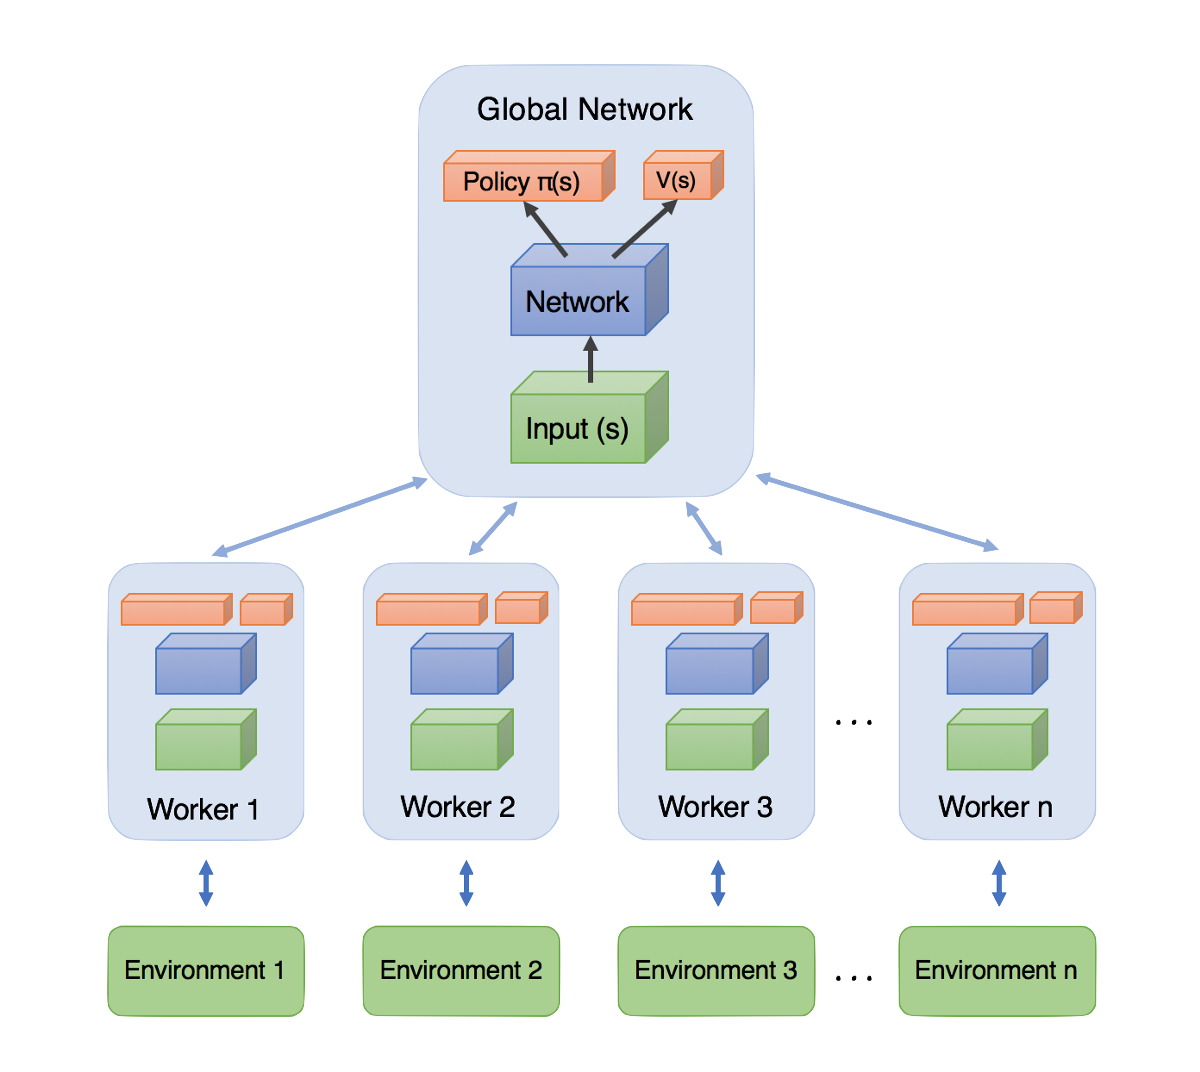
\includegraphics[width=.8\linewidth]{images/A3Carchitecture.png}
    \caption[High-level overview of the A3C algorithm]{High-level overview of the A3C algorithm. Each worker synchronizes its artificial neural network parameters with the global network and updates these based on input from the environment from which it is gathering transitions. Source: \cite{Juliani2016A3C}.}
    \label{fig:a3carchitecture}
\end{figure}
In $n$-step Q-learning and advantage actor-critic, a forward-view is used instead of the more commonly used backward view (which uses eligibility traces).
Forward view was found to be easier when training artificial neural networks with momentum-based methods and backpropagation through time.
To do this, we first compute a certain number of steps (or until the episode is over).
Then, the gradients are computed for each state-action pair encountered since the last update.
Each n-step update uses the longest possible n-step return resulting in a one-step update for the last state, a two-step update for the second last state, and so on for a total of up to the previously determined number of maximum allowed steps.
These accumulated gradients are then immediately applied to $\theta$.
This results in the pseudo-code shown in Algorithm~\ref{algo:a3c}.\\
\begin{algorithm}[htb]
\DontPrintSemicolon
\emph{// Assume global shared parameter vectors $\theta$ and $\theta_v$ and global shared counter $T=0$}\;
\emph{// Assume thread-specific parameter vectors $\theta'$ and $\theta'_v$}\;
Initialize thread step counter $t\gets 1$\;
\Repeat{$T > T_{max}$}{
    Reset gradients: $d\theta \gets 0$ and $d\theta_v \gets 0$\;
    Synchronize agent-specific parameters  $\theta'=\theta$ and $\theta'_v=\theta_v$\;
    $t_{start} \gets t$\;
    Initialize state $s_t$\;
    \Repeat{terminal $s_t$ \textbf{or} $t-t_{start}==t_{max}$}{
        Perform $a_t$ according to policy $\pi (a_t|s_t;\theta')$\;
        Receive reward $r_t$ and new state $s_{t+1}$\;
        $t \gets t + 1$\;
        $T \gets T + 1$\;
        }
        $R =
    \left\{
    \begin{array}{l l}
      0  \quad & \text{if $s_t$ is terminal}\\
        V(s_t,\theta'_v) \quad & \text{otherwise // Bootstrap from last state}
    \end{array}\right.$\;
    \For {$i \in \{t-1,\ldots,t_{start} \}$} {
        Accumulate gradients w.r.t. $\theta'$: $d\theta \gets d\theta + \nabla_{\theta'} \log\pi(a_i|s_i;\theta') (R - V(s_i;\theta'_v))$\;
        Accumulate gradients w.r.t. $\theta'_v$: $d\theta_v \gets d\theta_v + {\partial\left(R - V(s_i;\theta'_v)\right)^2}/{\partial \theta'_v}$\;
    }
    Perform asynchronous update of $\theta$ using $d\theta$ and of $\theta_v$ using $d\theta_v$\;
}
\caption[Asynchronous Advantage Actor Critic]{Asynchronous Advantage Actor Critic (A3C). Source: \cite{Mnih2016AsynchronousLearning}.}
\label{algo:a3c}
\end{algorithm}
% section deep_reinforcement_learning (end)
